\chapter{System Implementation}


This section presents the implementation details of the prototype system. The implementation follows the modular architecture introduced in the methodology section, where each subsystem is developed as an independent component and then connected to form the complete reporting pipeline.

The implementation focuses on building a functional prototype that can demonstrate the main reporting workflow. This includes citizen authentication, anonymous ticket-based report submission, backend relayer verification, AI-based text and image moderation, IPFS-based off-chain media storage, and smart contract anchoring on a private permissioned blockchain. The key performance and correctness aspects of these components are later evaluated in the testing and validation chapter.

\section{Permissioned Blockchain Implementation}

\begin{sloppypar}
The core infrastructure of the proposed system is the private permissioned blockchain network. The implementation focused on setting up a secure and efficient environment tailored for local governance applications.
\end{sloppypar}

\begin{itemize}
    \item {Geth \ac{PoA} Network Setup:} A private permissioned Ethereum-compatible network was initialized using the Go Ethereum client. The network was configured to operate in \ac{PoA} consensus mode, specifically using the Clique algorithm. This enabled faster block confirmation and lower energy consumption compared to traditional \ac{PoW} systems. A custom genesis file was created to define network parameters, including the initial set of authorized signers and the chain ID.
    
    \item {Validator Node Configuration:} Minimum of three full nodes were required to act as an validator. The 3 nodes are deployed in a personal \ac{VPS} infrastructure. Each node is configured with a unique cryptographic identity and their addresses were added to the list of authorized sealers within the consensus engine to manage transaction validation authority.

    \item {Network Security Measures:} To communicate with the blockchain network, secure \ac{RPC} endpoint was established for node 4. Node 4 is a non-validator node. Additionally, the network is configured to operate in a private subnet, further isolating it from external threats. This configuration allowed DApp and smart contracts to communicate with ledger enabling functions such as report submission, transaction querying and state synchronization.
\end{itemize}

The node configuration is shown in Figure~\ref{fig:validator_nodes}.


\begin{figure}[p]
    \centering
    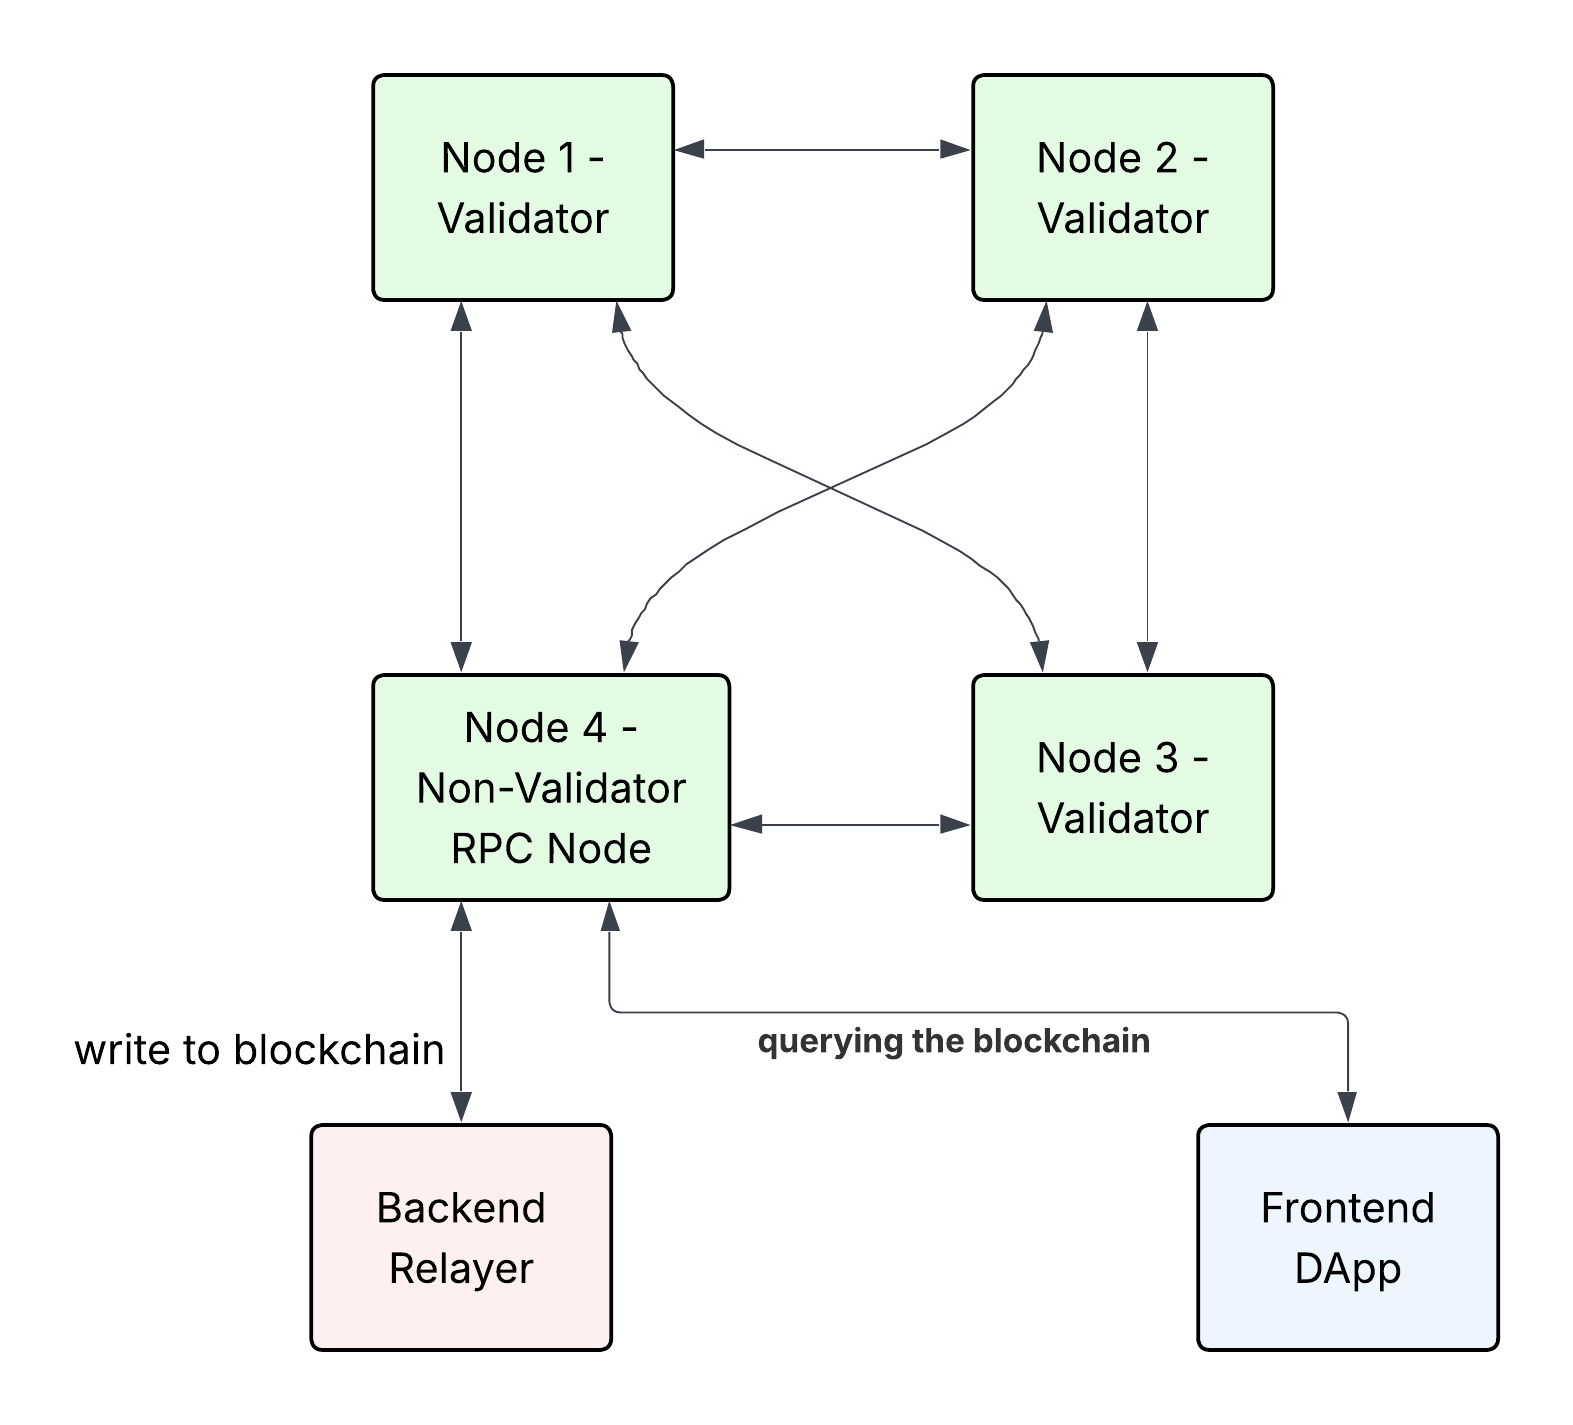
\includegraphics[max size={\textwidth}{\textheight}]{Images/Chapter 3/validator_nodes.png}
    \caption{Validator node configuration of the private permissioned blockchain.}
    \label{fig:validator_nodes}
\end{figure}

\section{Smart Contract Architecture and Logic}

The core on-chain logic of the decentralized reporting framework is governed by the Reporting.sol smart contract. This contract is designed to be highly gas-efficient, acting primarily as a state machine and a cryptographic ledger rather than a data storage layer. The implementation is divided into three critical functional domains as The Report Contract structure, Ticket Validation, and State Transition Logic.

\subsection{The Report Contract}
The Report Contract is engineered using a Separation of Concerns principle. To mitigate the prohibitive gas costs associated with storing large multimedia files on the blockchain, the contract only stores essential metadata. 
\begin{enumerate}
    \item Data Structure: Each civic issue is stored in a Report struct containing a unique integer ID, the IPFS \ac{CID} pointing to off-chain media, voting counters, the assigned authority address, and its current lifecycle state.
    \item \ac{RBAC}: Utilizing OpenZeppelin's AccessControl, the contract explicitly defines operational boundaries. The RELAYER\_ROLE is restricted to the backend server, allowing it to submit reports and relay votes on behalf of citizens. The AUTHORITY\_ROLE is granted to recognized government or NGO nodes, granting them permission to update an issue's status to solved or rejected.
\end{enumerate}

\subsection{Ticket Validation and Sybil Resistance}
A fundamental challenge in anonymous decentralized systems is preventing Sybil attacks and duplicate submissions. This framework utilizes a dual-layer validation mechanism based on Zero-Knowledge Proof \ac{ZKP} tickets.
\begin{enumerate}
    \item Off-Chain Cryptographic Validation: Before a transaction reaches the blockchain, the backend relayer intercepts the payload. Using ethers.js, it verifies that the zkpTicketId possesses a valid cryptographic signature from the official Government Authority. It subsequently verifies the citizen's signature against the payload hash to ensure data integrity during transmission.
    \item On-Chain Nullifier Tracking: Once validated off-chain, the zkpTicketId is passed to the smart contract as a submissionNullifier. The contract maintains a mapping of public submissionNullifiers. Upon successful report creation, this nullifier is marked as used. Any subsequent attempt to submit a report using the same ticket will systematically fail, cryptographically guaranteeing that one authorized ticket equates to exactly one unique report.
\end{enumerate}

\subsection{State Transition Logic}

\begin{figure}[!htbp]
    \centering
    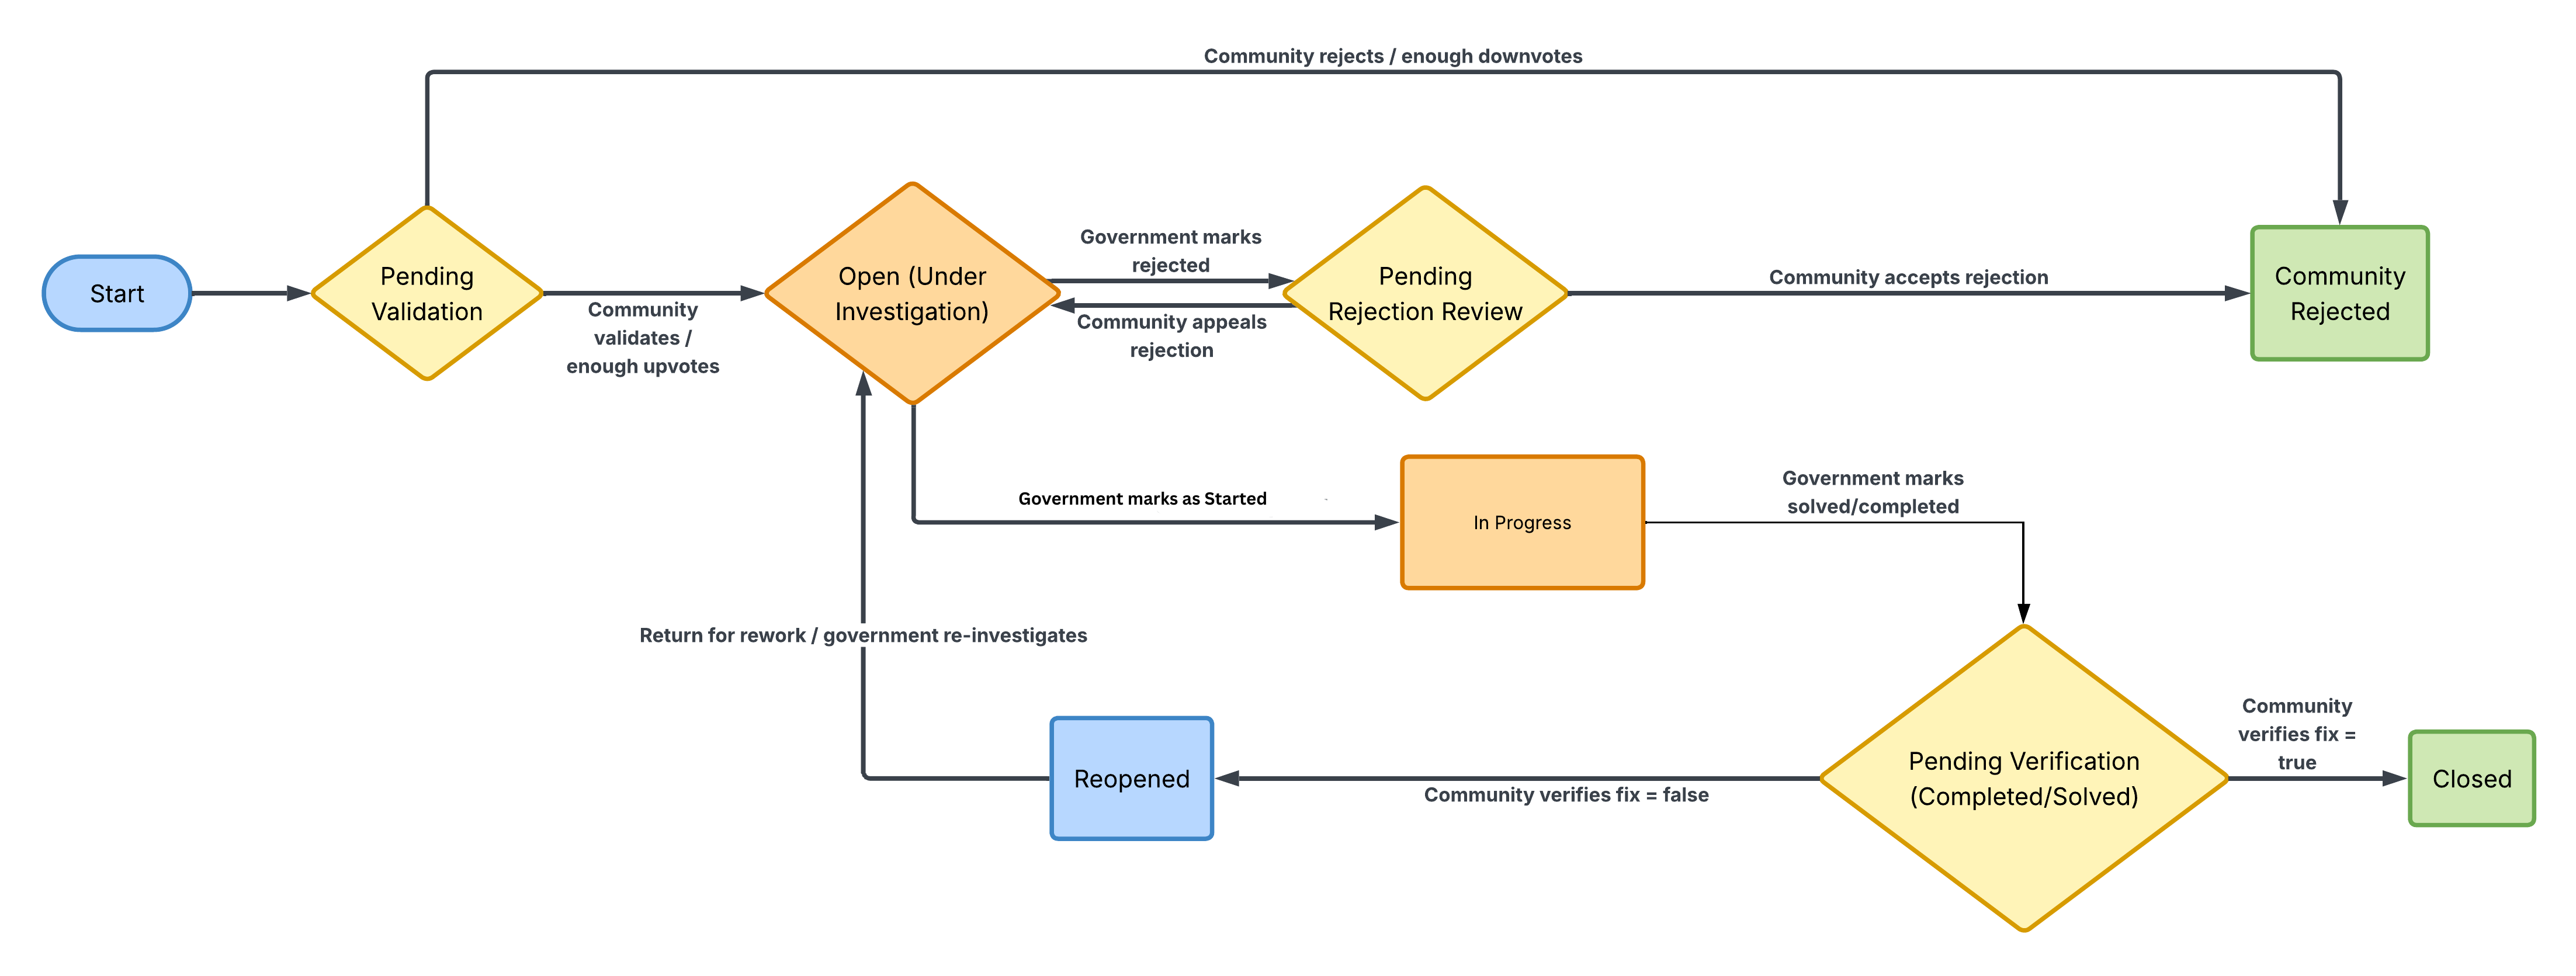
\includegraphics[width=\textwidth]{Images/Chapter 3/state-transition-diagram-3.png}
    \caption{State transition diagram for the civic reporting system.}
    \label{fig:state-transition}
\end{figure}

To enforce accountability and prevent solely rejection of civic issues by authorities, the contract implements a strict Finite State Machine (\ac{FSM}). Every submitted report strictly adheres to an 8-stage lifecycle managed via an on-chain enum:
\begin{enumerate}
    \item Pending Validation: Initial state awaiting community confirmation of legitimacy.
    \item Community Rejected: Terminal state for spam or invalid issues.
    \item Open: Validated by citizens and actively awaiting government action.
    \item In Progress: The authority has officially acknowledged the issue and is actively executing physical repairs or resolution steps.
    \item Pending Rejection Review: The authority dismissed the issue, triggering a community appeal phase.
    \item Pending Verification: The authority marked the active work as completed, triggering a mandatory community verification vote.
    \item Closed: Terminal state indicating a successfully verified resolution or an accepted rejection.
    \item Reopened: The community rejected the authority's fix, forcing the issue back to the authority for rework.
\end{enumerate}

A report must traverse these specific states driven by a combination of authority actions and community consensus thresholds.
\begin{enumerate}
    \item Community-Driven Transitions: When a report is submitted, it enters the Pending Validation state. The transition to the Open state (making it visible for government action) only occurs automatically via the \_changeStatus() function once the report receives a majority of upvotes from the community when time duration for voting ends.
    \item Authority-Driven Transitions: Authorities can only interact with reports in the Open, Reopened, or In Progress states. An authority calling startWork() shifts an Open or Reopened issue to the In Progress state, providing transparency to citizens that action is underway. From the In Progress state, calling markAsSolved() shifts the report to Pending Verification. Additionally, calling rejectIssue() from the Open or In Progress states shifts it to Pending Rejection Review.
    \item Consensus Verification: The FSM mandates that authority actions are never final until verified by the community. If an authority marks an issue as solved, the community must vote to verify the physical fix. If the majority votes to accept the fix, the report transitions to Closed. If the majority votes to reject the fix, the report transitions back to Reopened, signaling that further work is needed and allowing the community to continue monitoring the issue until a satisfactory resolution is achieved.
\end{enumerate}

\section{Identity and Access Control Implementation}

To satisfy the project's requirement for privacy-preserving accountability, an identity decoupling mechanism was successfully developed. This subsystem ensures that citizens can interact with the blockchain anonymously while remaining verified by an off-chain authority. The implementation was structured into three main components

\begin{itemize}
    \item {GovID Simulator:} An off-chain simulated identity server was developed and deployed to a personal \ac{VPS}. This service acts as the trusted authority for verifying real-world identities. A dedicated API endpoint (/api/govid/verify-citizen) was implemented to securely authenticate users via their National Identity Number (govId) and a password, bridging the gap between traditional web authentication and decentralized access.
    \item {Citizen Keypair generation:} To completely decouple a user's real identity from their on-chain footprint, the identity server does not store or transmit blockchain addresses. Instead, upon successful authentication, the simulator generates and returns a secure, 256-bit citizenSeed. This cryptographic seed is then used by the client-side DApp to deterministically generate an anonymous public-private keypair, allowing the citizen to interact securely with smart contracts without exposing personal data.
    \item {Ticket Batch Generation:} To facilitate multiple secure, anonymous report submissions over time, the simulator implements a batch authorization protocol. During authentication, the server generates a structured ticketBatch (currently configured to issue 10 tickets per request). Each ticket contains a unique ticketId (a cryptographic hash) and a signature signed by the Identity Authority's private key. Citizens use these single-use tickets to authorize their transactions on-chain. The backend relayer validates the authority's signature on the ticket, granting access without ever knowing which specific citizen is submitting the report.
\end{itemize}

\section{Backend Relayer Implementation}
The backend relayer serves as a critical middleware component that bridges the frontend DApp with the blockchain network and external services. It is responsible for handling report submissions, managing interactions with IPFS for off-chain storage, and orchestrating AI-based content moderation before anchoring data on the blockchain.

The implementation utilizes the NestJS framework to provide a robust and highly modular RESTful API. The core workflow of the relayer executes the following deterministic pipeline for each incoming citizen report.

\begin{figure}[!htbp]
    \centering
    \includegraphics[width=\textwidth,height=0.75\textheight,keepaspectratio]{Images/Chapter 3/backend-relayer-impl.png}
    \caption{Backend relayer workflow architecture.}
    \label{fig:backend-relayer-impl}
\end{figure}

\begin{enumerate}
    \item Cryptographic Verification: The relayer receives the payload via a POST /report endpoint. Utilizing the ethers.js library, it performs a strict dual-signature validation:
    \begin{enumerate}
        \item It verifies the ZKP Govid Simulator ticket signature against the dynamically fetched Government Authority public key to ensure the user is an authorized citizen.
        \item It reconstructs the payload hash (binding the description and ticket ID) and verifies the citizen's signature to prevent data tampering in transit.
    \end{enumerate}
    
    \item AI Content Moderation: To prevent on-chain spam, toxic immutability of blockchains and ensure platform integrity, the relayer routes the submitted text and media to the AI Oracle moderation service. This service acts as an automated filter, analyzing the content for appropriateness and returning a validation verdict before any storage operations occur.
    
    \item Decentralized Storage - \ac{IPFS}: To maintain a highly efficient and cost-effective blockchain state, heavy multimedia files and detailed text are offloaded to \ac{IPFS}. The relayer manages the file buffers via multer, processes the upload, and retrieves an immutable \ac{CID}.
    
    \item Gasless Blockchain Submission: As the final step, the relayer formats a transaction containing the IPFS CID and the ZKP ticket (which serves as a Sybil-resistant submissionNullifier). The relayer signs and dispatches this transaction to the Reporting.sol smart contract. By paying the network gas fees from its own wallet, the relayer enables a completely frictionless, gasless experience for the end-user.
\end{enumerate}

\section{IPFS Off-chain Storage Integration}


The system uses IPFS to store images. These images come from citizens who send reports. The images are not saved on the blockchain. Only a short code called a CID is saved there. The CID works like a fingerprint for the image. If anyone changes the image, the CID changes too. This keeps the images safe from tampering. It also keeps the blockchain from getting too full.

The IPFS part of the system is built in layers. Each layer has a job. One layer checks the image before it is stored. It makes sure the file is the right type and not too big. Another layer handles uploading and getting images back. There is also a layer that talks to the IPFS node directly.

When a citizen sends a report, the image goes to the backend server first. The server sends the image to an AI tool that checks if the image is okay. If the image passes the check, the server sends it to the IPFS part. The IPFS part saves the image and gives back a CID. The server takes that CID and adds it to the report. Then it sends everything to the blockchain.

When someone needs to see the image, the system reads the CID from the blockchain. It then uses the CID to retrieve the image. The image is shown in the app. Because the CID is derived from the image itself, the system can verify that the image was not changed.

The system also checks the CID before saving it to the blockchain. This makes sure the image can actually be found. The whole system runs inside Docker. It uses two containers. One is for the IPFS service. The other is for the IPFS node. The IPFS service is available on port 4000.

Right now the system uses only one IPFS node. In the future, three nodes will be used. Each node will be on a different machine. All three will be connected to each other. When an image is saved on one node, the other two will copy it. If one node stops working, the others still have the image. This makes the system more reliable. All of this will be done in a private network. It will not connect to the public IPFS network.


\subsection{AI-based Moderation System Implementation}


\begin{figure}[!htbp]
    \centering
    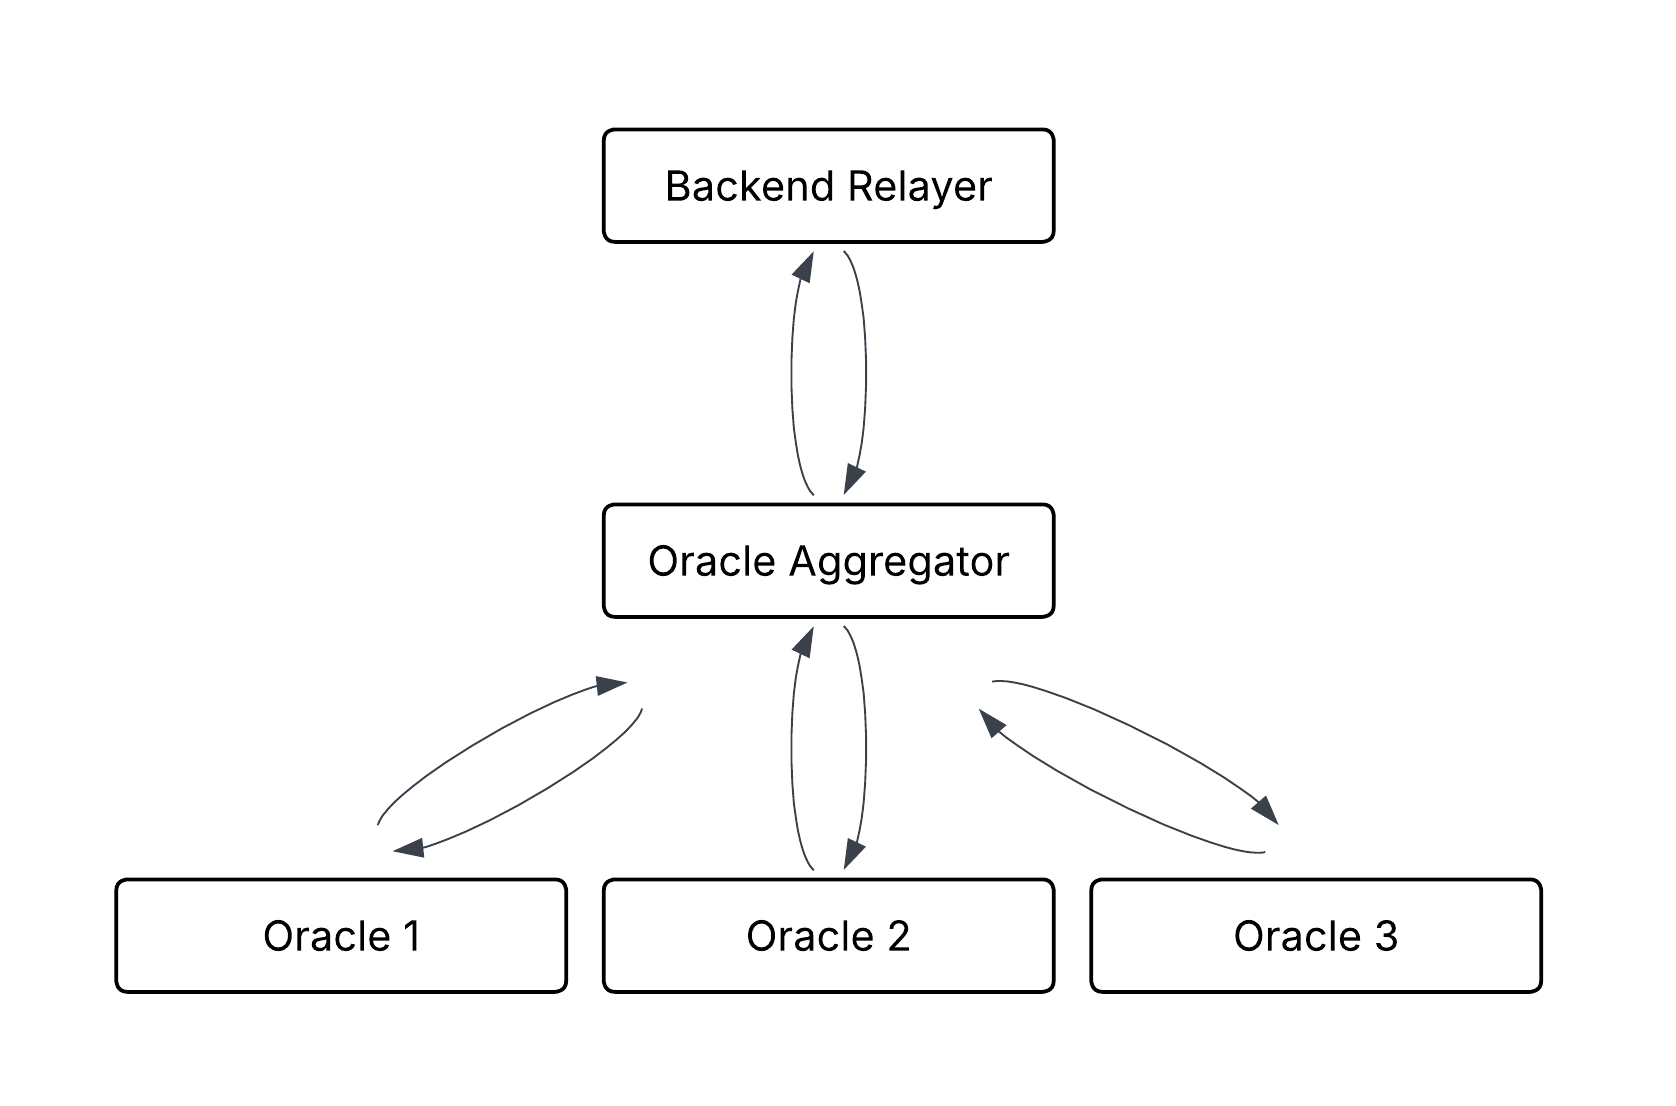
\includegraphics[width=\textwidth,height=0.75\textheight,keepaspectratio]{Images/Chapter_3/oracle-architecture.png}
    \caption{Oracle network architecture for AI moderation.}
    \label{fig:oracle-architecture}
\end{figure}

The AI moderation subsystem is implemented as an off-chain oracle service. It is placed between the backend relayer and the IPFS submission stage. This ensures that harmful, spam, irrelevant, or unsafe content is filtered before it is permanently stored or referenced by the blockchain.

The moderation service is designed as a containerized oracle network. It contains one aggregator service and three oracle worker services. The backend relayer communicates only with the aggregator. The aggregator then communicates with the oracle workers using internal Docker networking. This keeps the worker services isolated from public access and exposes only one controlled moderation API to the rest of the system.  This architecture is demonstrated in Figure~\ref{fig:oracle-architecture}.

The implemented oracle workers are as follows:

\begin{itemize}
    \item \textbf{Safety Oracle:} This oracle checks whether submitted text or images contain unsafe content. For text, it checks toxic, abusive, and threatening patterns using \texttt{unitary/toxic-bert}. For image moderation it uses pre-trained \texttt{Falconsai/nsfw\_image\_detection} to detect unsafe visual content.

    \item \textbf{Spam and Abuse Oracle:} This oracle checks whether the submitted report contains spam-like or low-quality text. It detects promotional phrases, repeated symbols, suspicious URLs, very short descriptions, and common spam patterns.It combines rule-based checks with lightweight NLP model \texttt{mrm8488/bert-tiny-finetuned-sms-spam-detection}.

    \item \textbf{Civic Relevance Oracle:} This oracle checks whether the submitted
    report is related to a public or local governance issue. It uses sentence-transformer model \texttt{sentence-transformers/all-MiniLM-L6-v2} to compare the report text against predefined civic issue descriptions, such as road damage, waste management, drainage, water supply, streetlights, flooding, traffic safety, public property damage, and environmental issues.
\end{itemize}


Each oracle returns a structured vote containing the oracle identifier, vote, confidence value, explanation code, model or rule version, and additional details. The accepted vote values are ACCEPT and REJECT. The system does not currently use a manual REVIEW state because that would introduce a central human moderation dependency. Instead, unclear or low-quality reports are rejected and the citizen can resubmit a clearer report.

The aggregator combines the oracle outputs using a rule-based decision strategy. If a critical safety violation is detected, the final decision is REJECT. If the civic relevance oracle identifies the content as non-civic, the final decision is also REJECT. Otherwise, the aggregator applies majority voting among the three oracles. If at least two oracle workers accept the content, the final result is ACCEPT. If not, the final result is REJECT.

Security and integrity are also included in the moderation workflow. The backend relayer signs the moderation request using its private wallet key. The aggregator recovers the signer address from the relayer signature and compares it with the trusted relayer address configured in the oracle environment. The request also includes a timestamp and nonce. The timestamp prevents stale requests, while the
nonce prevents replay attacks. The aggregator computes a report hash and a decision hash, signs the final decision, and returns this information to the relayer. This makes the moderation result tamper-evident and auditable.

The AI moderation service is deployed on a VPS using Docker containers managed through Dokploy. The deployment consists of the oracle aggregator, safety oracle, spam and abuse oracle, and civic relevance oracle containers. At the current stage, the service has been integrated with the backend relayer and supports both text-based moderation and image safety moderation during the report submission
workflow.




\subsection{Web-based DApp Development}
The decentralized application (DApp) serves as the primary gateway for citizens to interact with the local governance system. It is built using a modern web stack comprising Next.js and React for the frontend interface, Tailwind CSS for responsive styling, and Ethers.js for cryptographic operations. The architecture is designed to abstract blockchain complexities away from the end-user while maintaining strict privacy and security guarantees.

\subsubsection*{User Authentication Interface}
The authentication interface is designed to verify citizen eligibility without compromising personal privacy.
\begin{itemize}
    \item \textbf{GovID Verification Integration:} The interface securely collects the citizen's GovID credentials and interfaces with an external GovID Simulator API. This abstracts the process of verifying a citizen's real-world identity against a centralized registry.
    \item \textbf{Cryptographic Credential Generation:} Upon successful identity verification, the system retrieves a batch of \ac{ZKP} tickets and a unique `citizenSeed`. 
    \item \textbf{Local State Management:} Using the `ethers.js` library, a localized Citizen Wallet is derived from the seed. A custom React Context (\texttt{CitizenContext}) is utilized to manage the session state, ensuring that the generated private keys and ZKP tickets remain strictly on the client-side device and are never exposed to external servers. The UI incorporates dynamic feedback mechanisms to indicate the generation of cryptographic proofs to the user.
\end{itemize}

\subsubsection*{Report Submission Interface}
The report submission module allows authenticated citizens to report civic issues anonymously.
\begin{itemize}
    \item \textbf{Form Design and Data Handling:} Developed with a mobile-first approach, the form captures issue descriptions and optional photographic evidence using standard \texttt{FormData} structures to support multipart uploads.
    \item \textbf{Anonymous Cryptographic Signing:} To guarantee anonymity and prevent spam, each submission consumes a single ZKP ticket from the user's allocated batch. The payload (consisting of the issue description and the ZKP ticket ID) is hashed using Keccak-256 and subsequently signed using the citizen's locally stored ECDSA private key.
    \item \textbf{Meta-Transaction Relaying:} Instead of submitting transactions directly to the blockchain and incurring gas fees, the frontend dispatches the signed payload, image, and ZKP metadata to a NestJS Backend Relayer. The relayer handles the intermediate steps: uploading the evidence to IPFS, requesting AI moderation, and finally submitting the transaction to the Geth blockchain network on behalf of the user.
\end{itemize}

\subsubsection*{Blockchain Query Interface}
The query interface acts as a community feed where citizens can view, filter, and track the status of reported issues.
\begin{itemize}
    \item \textbf{Mobile-First Feed Architecture:} Implemented as a single-column, scrollable interface inspired by modern social media platforms (e.g., Reddit). This design choice prioritizes readability and user engagement on mobile devices.
    \item \textbf{Dynamic Issue Cards:} Data retrieved from the blockchain is formatted into interactive cards. Each card displays critical metadata including categorical status badges (e.g., PENDING VALIDATION, OPEN, RESOLVED), community upvotes, truncated descriptions, timestamps, and image thumbnails.
    \item \textbf{State Management and Navigation:} The interface employs React state hooks to allow real-time filtering of issues by category (e.g., Infrastructure, Parks \& Rec, Safety). Furthermore, a persistent Floating Action Button (FAB) is implemented to provide users with seamless access to the report submission workflow at any time.
\end{itemize}

% \subsection{Deployment Environment}

% Very important.

% Discuss:

% VPS infrastructure,
% Ubuntu server,
% Docker containers,
% service distribution.

% Include deployment diagram.
